\documentclass[aspectratio=43]{beamer}

% Theme and color scheme
\usetheme{Madrid}
\usecolortheme{default}

% Packages
\usepackage[utf8]{inputenc}
\usepackage[T1]{fontenc}
\usepackage{graphicx}
\usepackage{amsmath}
\usepackage{amsfonts}
\usepackage{amssymb}
\usepackage{hyperref}
\usepackage{multicol}
\usepackage{tikz}
\usepackage{xcolor}

% Custom colors
\definecolor{uniblue}{RGB}{0,51,102}
\definecolor{highlight}{RGB}{255,153,0}

% Environmental gradient colors (define globally)
\definecolor{envlow}{RGB}{255,245,235}     % Light orange
\definecolor{envmed}{RGB}{253,174,97}      % Medium orange
\definecolor{envhigh}{RGB}{215,48,31}      % Dark red

% Set theme colors
\setbeamercolor{structure}{fg=uniblue}
\setbeamercolor{frametitle}{bg=white,fg=black}

% Custom headline: white background + thin uniblue line at the bottom
\setbeamertemplate{frametitle}{
  \nointerlineskip
  \begin{beamercolorbox}[wd=\paperwidth,ht=2.5ex,dp=1ex,left]{frametitle}
    \hspace*{2em} % Move text right
    \vspace*{-1.5ex}\strut\insertframetitle\strut
  \end{beamercolorbox}
  \hspace*{-2em} % Move line right
  {\color{uniblue}\rule{\paperwidth}{0.7mm}}
}

% Remove navigation symbols
\setbeamertemplate{navigation symbols}{}

% Remove footline
\setbeamertemplate{footline}{}

% Custom title page
\setbeamertemplate{title page}{
    \begin{picture}(0,0)
        \put(25,-220){
\includegraphics[width=0.8\paperwidth]{Imgs/Loghi.png}}
    \end{picture}
    \vfill
    \centering
    \begin{beamercolorbox}[sep=8pt,center]{title}
        \usebeamerfont{title}\inserttitle\par%
        \ifx\insertsubtitle\@empty%
        \else%
            \vskip0.25em%
            {\usebeamerfont{subtitle}\usebeamercolor[fg]{subtitle}\insertsubtitle\par}%
        \fi%
    \end{beamercolorbox}%
    \vskip1em\par
    \begin{beamercolorbox}[sep=8pt,center]{author}
        \usebeamerfont{author}\insertauthor
    \end{beamercolorbox}
    \begin{beamercolorbox}[sep=8pt,center]{institute}
        \usebeamerfont{institute}\insertinstitute
    \end{beamercolorbox}
    \begin{beamercolorbox}[sep=8pt,center]{date}
        \usebeamerfont{date}\insertdate
    \end{beamercolorbox}\vskip0.5em
    \vfill
}

% Document information
\title{Geomatic Techniques to Support Phytosanitary Products Tests whithin the EPPO Standard Framework}
\author{Samuele Bumbaca}
\institute{University of Turin}
\date{August 28, 2025}

\begin{document}

% Title slide
\begin{frame}
    \titlepage
\end{frame}

% Slide 2: The Traditional Approach to Agricultural Trials
\begin{frame}
    \frametitle{The Traditional Approach to Agricultural Trials}
    
    \begin{columns}
        \begin{column}{0.65\textwidth}
            \begin{center}
                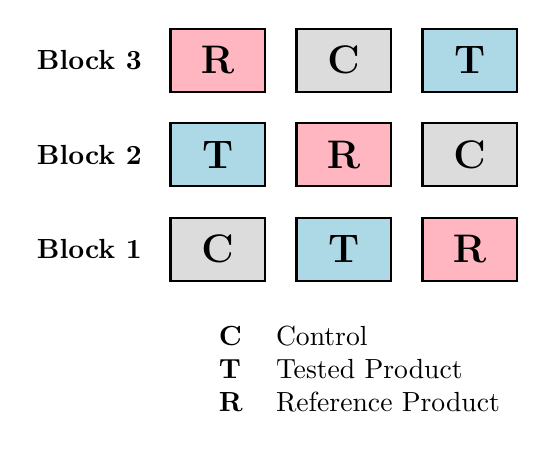
\begin{tikzpicture}[scale=0.8]
                    % Define colors for treatments
                    \definecolor{control}{RGB}{220,220,220}
                    \definecolor{tested}{RGB}{173,216,230}
                    \definecolor{reference}{RGB}{255,182,193}
                    
                    % Draw grid and plots
                    \foreach \row in {0,1,2} {
                        \foreach \col in {0,1,2} {
                            % Calculate position
                            \pgfmathsetmacro{\x}{\col*2}
                            \pgfmathsetmacro{\y}{\row*1.5}
                            
                            % Assign treatments (Latin square-like design)
                            \pgfmathsetmacro{\treatment}{int(mod(\col + \row, 3))}
                            \ifnum\treatment=0
                                \def\plotcolor{control}
                                \def\plotlabel{C}
                            \fi
                            \ifnum\treatment=1
                                \def\plotcolor{tested}
                                \def\plotlabel{T}
                            \fi
                            \ifnum\treatment=2
                                \def\plotcolor{reference}
                                \def\plotlabel{R}
                            \fi
                            
                            % Draw plot
                            \fill[\plotcolor] (\x,\y) rectangle (\x+1.5,\y+1);
                            \draw[black, thick] (\x,\y) rectangle (\x+1.5,\y+1);
                            \node at (\x+0.75,\y+0.5) {\Large\textbf{\plotlabel}};
                        }
                        % Block labels
                        \node[left] at (-0.3,\row*1.5+0.5) {\textbf{Block \pgfmathprint{int(\row+1)}}};
                    }
                    
                    % Legend
                    \node[below] at (3,-0.5) {
                        \begin{tabular}{ll}
                            \textbf{C} & Control \\
                            \textbf{T} & Tested Product \\
                            \textbf{R} & Reference Product
                        \end{tabular}
                    };
                \end{tikzpicture}
            \end{center}
        \end{column}
        
        \begin{column}{0.35\textwidth}
            \begin{block}{ANOVA Model:}
                \begin{equation*}
                    y_{ij} = \mu + \alpha_i + \beta_j + \varepsilon_{ij}
                \end{equation*}
                
                \small
                Where:
                \begin{itemize}
                    \item $y_{ij}$ = response
                    \item $\mu$ = overall mean
                    \item $\alpha_i$ = treatment effect
                    \item $\beta_j$ = block effect
                    \item $\varepsilon_{ij}$ = random error
                \end{itemize}
            \end{block}
            
            \begin{alertblock}{\tiny Note:}
                {\tiny This is the \textbf{additive model}. Modern approaches may include interaction terms: $\alpha_i \times \beta_j$}
            \end{alertblock}
        \end{column}
    \end{columns}
\end{frame}

% Slide 3: Key Assumptions of Traditional ANOVA
\begin{frame}
    \frametitle{Key Assumptions of Traditional ANOVA}
    
    \begin{block}{Statistical Assumptions:}
        \begin{itemize}
            \item \textbf{Randomization}: Treatments randomly assigned within blocks
            \item \textbf{Replication}: Each treatment appears in each block
            \item \textbf{Independence}: Observations are independent given the design
            \item \textbf{Homoscedasticity }: Equal variances across treatments
            \item \textbf{Normality}: Residuals follow normal distribution
        \end{itemize}
    \end{block}

    \begin{alertblock}{Consequences of Assumption Violations:}
        \begin{itemize}
            \item \textbf{Invalid conclusions of parametric tests}: Need for non-parametric tests leading to reduced statistical power
        \end{itemize}
    \end{alertblock}
    
    \vfill
    {\tiny
    \begin{flushleft}
        Based on R. A. Fisher, Statistical Methods for Research Workers, in S. Kotz \& N. L. Johnson (eds.), Breakthroughs in Statistics: Methodology and Distribution, pp. 66--70, Springer, New York, 1992.
    \end{flushleft}
    }
\end{frame}

% Slide 4: Right Blocking
\begin{frame}
    \frametitle{The Right Blocking: Capturing Environmental Variability}
    
    \begin{columns}
        \begin{column}{0.7\textwidth}
            \begin{center}
                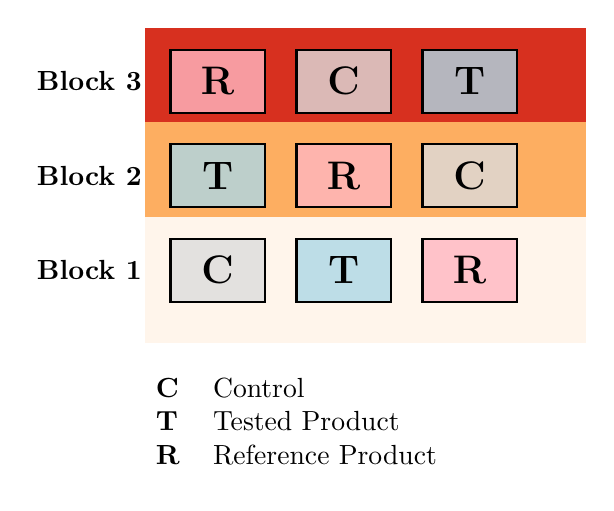
\begin{tikzpicture}[scale=0.8]
                    % Define colors for treatments
                    \definecolor{control}{RGB}{220,220,220}
                    \definecolor{tested}{RGB}{173,216,230}
                    \definecolor{reference}{RGB}{255,182,193}
                    
                    % Draw environmental variability strips (background)
                    \def\xoffset{0.1}
                    \def\yoffset{-0.15}
                    \fill[envlow] ({-0.5+\xoffset},{-0.5+\yoffset}) rectangle ({6.5+\xoffset},{1.5+\yoffset});
                    \fill[envmed] ({-0.5+\xoffset},{1.5+\yoffset}) rectangle ({6.5+\xoffset},{3+\yoffset});
                    \fill[envhigh] ({-0.5+\xoffset},{3+\yoffset}) rectangle ({6.5+\xoffset},{4.5+\yoffset});
                    
                    % Draw grid and plots
                    \foreach \row in {0,1,2} {
                        \foreach \col in {0,1,2} {
                            % Calculate position
                            \pgfmathsetmacro{\x}{\col*2}
                            \pgfmathsetmacro{\y}{\row*1.5}
                            
                            % Assign treatments (Latin square-like design)
                            \pgfmathsetmacro{\treatment}{int(mod(\col + \row, 3))}
                            \ifnum\treatment=0
                                \def\plotcolor{control}
                                \def\plotlabel{C}
                            \fi
                            \ifnum\treatment=1
                                \def\plotcolor{tested}
                                \def\plotlabel{T}
                            \fi
                            \ifnum\treatment=2
                                \def\plotcolor{reference}
                                \def\plotlabel{R}
                            \fi
                            
                            % Draw plot with some transparency to show environment
                            \fill[\plotcolor,opacity=0.8] (\x,\y) rectangle (\x+1.5,\y+1);
                            \draw[black, thick] (\x,\y) rectangle (\x+1.5,\y+1);
                            \node at (\x+0.75,\y+0.5) {\Large\textbf{\plotlabel}};
                        }
                        % Block labels
                        \node[left] at (-0.3,\row*1.5+0.5) {\textbf{Block \pgfmathprint{int(\row+1)}}};
                    }
                    
                    % Legend for treatments
                    \node[below] at (2,-1) {
                        \begin{tabular}{ll}
                            \textbf{C} & Control \\
                            \textbf{T} & Tested Product \\
                            \textbf{R} & Reference Product
                        \end{tabular}
                    };
                \end{tikzpicture}
            \end{center}
        \end{column}
        
        \begin{column}{0.3\textwidth}
            \begin{block}{\small Environmental Gradient:}
                \scriptsize
                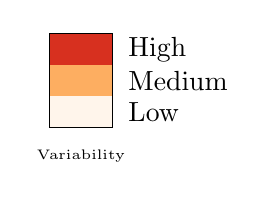
\begin{tikzpicture}[scale=0.8]
                    % Color scale bar
                    \fill[envlow] (0,0) rectangle (1,0.5);
                    \fill[envmed] (0,0.5) rectangle (1,1);
                    \fill[envhigh] (0,1) rectangle (1,1.5);
                    \draw[black] (0,0) rectangle (1,1.5);
                    
                    % Labels
                    \node[right] at (1.1,0.25) {Low};
                    \node[right] at (1.1,0.75) {Medium};
                    \node[right] at (1.1,1.25) {High};
                    \node[below] at (0.5,-0.2) {\tiny Variability};
                \end{tikzpicture}
            \end{block}
        \end{column}
    \end{columns}
    
    \begin{exampleblock}{\small Success of Blocking Strategy:}
        \begin{itemize}
            \scriptsize
            \item \textbf{Within-block homogeneity}: Treatments compared under similar conditions
            \item \textbf{Between-block heterogeneity}: Environmental gradient captured by block effects
        \end{itemize}
    \end{exampleblock}
\end{frame}

% Slide 5: The Wrong Blocking
\begin{frame}
    \frametitle{The Wrong Blocking: Assumption Violation}
    
    \begin{columns}
        \begin{column}{0.7\textwidth}
            \begin{center}
                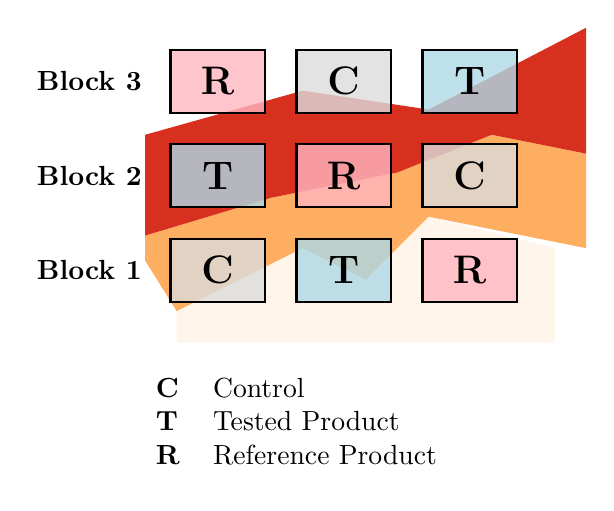
\begin{tikzpicture}[scale=0.8]
                    % Define colors for treatments
                    \definecolor{control}{RGB}{220,220,220}
                    \definecolor{tested}{RGB}{173,216,230}
                    \definecolor{reference}{RGB}{255,182,193}
                    
                    % Draw irregular environmental variability shapes (background)
                    \def\xoffset{0.1}
                    \def\yoffset{-0.15}
                    
                    % Irregular environmental patches that don't align with blocks
                    % Low variability (diagonal patches)
                    \fill[envlow] ({0+\xoffset},{0+\yoffset}) -- ({2+\xoffset},{1+\yoffset}) -- ({3+\xoffset},{0.5+\yoffset}) -- ({4+\xoffset},{1.5+\yoffset}) -- ({6+\xoffset},{1+\yoffset}) -- ({6+\xoffset},{-0.5+\yoffset}) -- ({0+\xoffset},{-0.5+\yoffset}) -- cycle;
                    
                    % Medium variability (curved patches)
                    \fill[envmed] ({-0.5+\xoffset},{1.2+\yoffset}) -- ({1.5+\xoffset},{1.8+\yoffset}) -- ({3.5+\xoffset},{2.2+\yoffset}) -- ({5+\xoffset},{2.8+\yoffset}) -- ({6.5+\xoffset},{2.5+\yoffset}) -- ({6.5+\xoffset},{1+\yoffset}) -- ({4+\xoffset},{1.5+\yoffset}) -- ({3+\xoffset},{0.5+\yoffset}) -- ({2+\xoffset},{1+\yoffset}) -- ({0+\xoffset},{0+\yoffset}) -- ({-0.5+\xoffset},{0.8+\yoffset}) -- cycle;
                    
                    % High variability (irregular top patches)
                    \fill[envhigh] ({-0.5+\xoffset},{2.8+\yoffset}) -- ({2+\xoffset},{3.5+\yoffset}) -- ({4+\xoffset},{3.2+\yoffset}) -- ({6.5+\xoffset},{4.5+\yoffset}) -- ({6.5+\xoffset},{2.5+\yoffset}) -- ({5+\xoffset},{2.8+\yoffset}) -- ({3.5+\xoffset},{2.2+\yoffset}) -- ({1.5+\xoffset},{1.8+\yoffset}) -- ({-0.5+\xoffset},{1.2+\yoffset}) -- cycle;
                    
                    % Draw grid and plots
                    \foreach \row in {0,1,2} {
                        \foreach \col in {0,1,2} {
                            % Calculate position
                            \pgfmathsetmacro{\x}{\col*2}
                            \pgfmathsetmacro{\y}{\row*1.5}
                            
                            % Assign treatments (Latin square-like design)
                            \pgfmathsetmacro{\treatment}{int(mod(\col + \row, 3))}
                            \ifnum\treatment=0
                                \def\plotcolor{control}
                                \def\plotlabel{C}
                            \fi
                            \ifnum\treatment=1
                                \def\plotcolor{tested}
                                \def\plotlabel{T}
                            \fi
                            \ifnum\treatment=2
                                \def\plotcolor{reference}
                                \def\plotlabel{R}
                            \fi
                            
                            % Draw plot with some transparency to show environment
                            \fill[\plotcolor,opacity=0.8] (\x,\y) rectangle (\x+1.5,\y+1);
                            \draw[black, thick] (\x,\y) rectangle (\x+1.5,\y+1);
                            \node at (\x+0.75,\y+0.5) {\Large\textbf{\plotlabel}};
                        }
                        % Block labels
                        \node[left] at (-0.3,\row*1.5+0.5) {\textbf{Block \pgfmathprint{int(\row+1)}}};
                    }
                    
                    % Legend for treatments
                    \node[below] at (2,-1) {
                        \begin{tabular}{ll}
                            \textbf{C} & Control \\
                            \textbf{T} & Tested Product \\
                            \textbf{R} & Reference Product
                        \end{tabular}
                    };
                \end{tikzpicture}
            \end{center}
        \end{column}
        
        \begin{column}{0.3\textwidth}
            \begin{block}{\small Environmental Gradient:}
                \scriptsize
                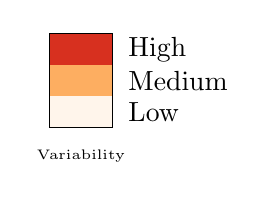
\begin{tikzpicture}[scale=0.8]
                    % Color scale bar
                    \fill[envlow] (0,0) rectangle (1,0.5);
                    \fill[envmed] (0,0.5) rectangle (1,1);
                    \fill[envhigh] (0,1) rectangle (1,1.5);
                    \draw[black] (0,0) rectangle (1,1.5);
                    
                    % Labels
                    \node[right] at (1.1,0.25) {Low};
                    \node[right] at (1.1,0.75) {Medium};
                    \node[right] at (1.1,1.25) {High};
                    \node[below] at (0.5,-0.2) {\tiny Variability};
                \end{tikzpicture}
            \end{block}
        \end{column}
    \end{columns}
    
    \begin{alertblock}{\small Heteroscedasticity Assumption Violation Problem:}
        \scriptsize
        \begin{itemize}
            \item \textbf{Blocks fail to capture environmental variability}: Treatments compared under different conditions
            \item \textbf{Invalid parametric test}: Residual variance differs across treatments
        \end{itemize}
    \end{alertblock}
\end{frame}

% Slide 6: The Problem
\begin{frame}
    \frametitle{Current Limitations in Statistics for Agricultural Trials}
    
    \begin{block}{Traditional Approach Issues:}
        \begin{itemize}
            \item \textbf{Human-dependent blocking}: Environmental variability assessment relies on experimenter experience
            \item \textbf{A priori identification}: Must identify variance sources BEFORE data collection
        \end{itemize}
    \end{block}
    
    \begin{alertblock}{The Challenge:}
        \textit{How can we capture environmental variability mathematically rather than through human judgment?}
    \end{alertblock}
\end{frame}

% Slide 7: Geostatistical Approach
\begin{frame}
    \frametitle{Geostatistical Approach: Spatial Linear Mixed Models}
    
    \begin{columns}
        \begin{column}{0.65\textwidth}
            \begin{center}
                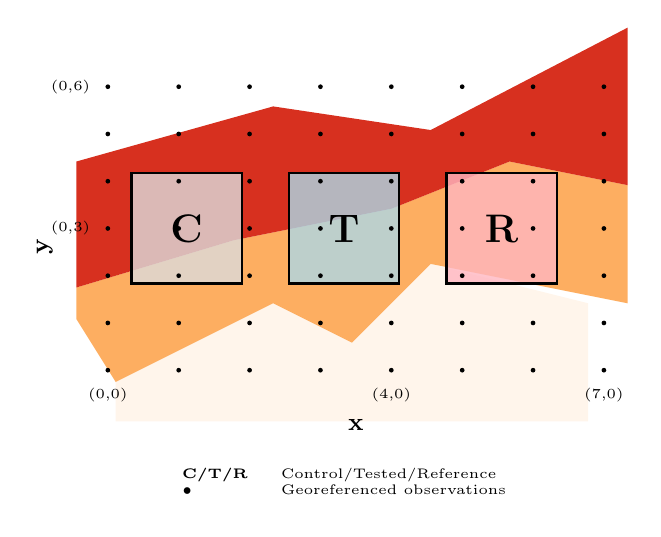
\begin{tikzpicture}[scale=1]
                    % Define colors for treatments
                    \definecolor{control}{RGB}{220,220,220}
                    \definecolor{tested}{RGB}{173,216,230}
                    \definecolor{reference}{RGB}{255,182,193}
                    
                    % Draw irregular environmental variability shapes (background)
                    \def\xoffset{0.1}
                    \def\yoffset{-0.15}
                    
                    % Same irregular environmental patches as slide 5
                    \fill[envlow] ({0+\xoffset},{0+\yoffset}) -- ({2+\xoffset},{1+\yoffset}) -- ({3+\xoffset},{0.5+\yoffset}) -- ({4+\xoffset},{1.5+\yoffset}) -- ({6+\xoffset},{1+\yoffset}) -- ({6+\xoffset},{-0.5+\yoffset}) -- ({0+\xoffset},{-0.5+\yoffset}) -- cycle;
                    
                    \fill[envmed] ({-0.5+\xoffset},{1.2+\yoffset}) -- ({1.5+\xoffset},{1.8+\yoffset}) -- ({3.5+\xoffset},{2.2+\yoffset}) -- ({5+\xoffset},{2.8+\yoffset}) -- ({6.5+\xoffset},{2.5+\yoffset}) -- ({6.5+\xoffset},{1+\yoffset}) -- ({4+\xoffset},{1.5+\yoffset}) -- ({3+\xoffset},{0.5+\yoffset}) -- ({2+\xoffset},{1+\yoffset}) -- ({0+\xoffset},{0+\yoffset}) -- ({-0.5+\xoffset},{0.8+\yoffset}) -- cycle;
                    
                    \fill[envhigh] ({-0.5+\xoffset},{2.8+\yoffset}) -- ({2+\xoffset},{3.5+\yoffset}) -- ({4+\xoffset},{3.2+\yoffset}) -- ({6.5+\xoffset},{4.5+\yoffset}) -- ({6.5+\xoffset},{2.5+\yoffset}) -- ({5+\xoffset},{2.8+\yoffset}) -- ({3.5+\xoffset},{2.2+\yoffset}) -- ({1.5+\xoffset},{1.8+\yoffset}) -- ({-0.5+\xoffset},{1.2+\yoffset}) -- cycle;
                    
                    % Add treatment rectangles in center Y of plot (larger rectangles)
                    \pgfmathsetmacro{\midY}{1.8}
                    \fill[color=control,opacity=0.8] (0.3,\midY-0.7) rectangle (1.7,\midY+0.7);
                    \draw[black, thick] (0.3,\midY-0.7) rectangle (1.7,\midY+0.7);
                    \node at (1,\midY) {\Large\textbf{C}};
                    
                    \fill[color=tested,opacity=0.8] (2.3,\midY-0.7) rectangle (3.7,\midY+0.7);
                    \draw[black, thick] (2.3,\midY-0.7) rectangle (3.7,\midY+0.7);
                    \node at (3,\midY) {\Large\textbf{T}};
                    
                    \fill[color=reference,opacity=0.8] (4.3,\midY-0.7) rectangle (5.7,\midY+0.7);
                    \draw[black, thick] (4.3,\midY-0.7) rectangle (5.7,\midY+0.7);
                    \node at (5,\midY) {\Large\textbf{R}};
                    
                    % Draw grid of observation points with coordinates (denser grid)
                    \foreach \row in {0,1,2,3,4,5,6} {
                        \foreach \col in {0,1,2,3,4,5,6,7} {
                            % Calculate position (adjusted for denser grid)
                            \pgfmathsetmacro{\x}{\col*0.9}
                            \pgfmathsetmacro{\y}{\row*0.6}
                            
                            % Draw observation point
                            \fill[black] (\x,\y) circle (0.03);
                            
                            % Add coordinate labels for some points (adjusted for new grid)
                            \ifnum\row=0
                                \ifnum\col=0
                                    \node[below, font=\tiny] at (\x,\y-0.1) {(0,0)};
                                \fi
                                \ifnum\col=4
                                    \node[below, font=\tiny] at (\x,\y-0.1) {(4,0)};
                                \fi
                                \ifnum\col=7
                                    \node[below, font=\tiny] at (\x,\y-0.1) {(7,0)};
                                \fi
                            \fi
                            \ifnum\col=0
                                \ifnum\row=3
                                    \node[left, font=\tiny] at (\x-0.1,\y) {(0,3)};
                                \fi
                                \ifnum\row=6
                                    \node[left, font=\tiny] at (\x-0.1,\y) {(0,6)};
                                \fi
                            \fi
                        }
                    }
                    
                    % Axis labels
                    \node[below, font=\small] at (3.15,-0.5) {\textbf{x}};
                    \node[left, font=\small, rotate=90] at (-0.8,1.8) {\textbf{y}};
                    
                    % Legend for treatments and spatial data
                    \node[below, font=\tiny] at (3,-1.1) {
                        \begin{tabular}{ll}
                            \textbf{C/T/R} & Control/Tested/Reference \\
                            \textbf{\(\bullet\)} & Georeferenced observations
                        \end{tabular}
                    };

                \end{tikzpicture}
            \end{center}
        \end{column}
        
        \begin{column}{0.35\textwidth}
            \begin{block}{\small Spatial LMM:}
                \begin{equation*}
                    y(s_i) = \mu + \alpha_j + f(s_i) + \varepsilon_i
                \end{equation*}
                
                \scriptsize
                Where:
                \begin{itemize}
                    \item $y(s_i)$ = response at $s_i$
                    \item $\mu$ = overall mean
                    \item $\alpha_j$ = treatment effect
                    \item $f(s_i)$ = spatial random field
                    \item $\varepsilon_i$ = error
                    \item $s_i = (x_i, y_i)$  = coordinates
                \end{itemize}
            \end{block}
            
        \end{column}
    \end{columns}
    
    \begin{exampleblock}{\scriptsize Benefits:}
        \tiny
        \begin{itemize}
            \item \textbf{No blocking}: Spatial correlation captures variability
            \item \textbf{Post-hoc}: No a priori variance identification
            \item \textbf{Homoscedasticity}: Assumption satisfied in more cases in respect blocking
        \end{itemize}
    \end{exampleblock}
\end{frame}

% Slide 8: Research Gap
\begin{frame}
    \frametitle{The Missing Link: Spatial Coordinates}
    
    \begin{columns}
        \begin{column}{0.5\textwidth}
            \begin{block}{Geostatistical Methods Advantages:}
                \begin{itemize}
                    \item[\textcolor{green}{\checkmark}] \textbf{Mathematical modeling} of environmental variability
                    \item[\textcolor{green}{\checkmark}] \textbf{Post-hoc analysis} - no need for prior knowledge of the environment variables and of their distribution
                    \item[\textcolor{green}{\checkmark}] \textbf{Superior performance} in handling spatial heterogeneity
                    \item[\textcolor{green}{\checkmark}] \textbf{EPPO recognized} approach
                \end{itemize}
            \end{block}
        \end{column}
        
        \begin{column}{0.5\textwidth}
            \begin{alertblock}{Current Barrier:}
                \begin{itemize}
                    \item[\textcolor{red}{\(\times\)}] \textbf{Requires spatially referenced observations}
                    \item[\textcolor{red}{\(\times\)}] \textbf{Traditional manual assessments lack coordinates}
                    \item[\textcolor{red}{\(\times\)}] \textbf{Implementation gap} in practical field trials
                \end{itemize}
            \end{alertblock}
        \end{column}
    \end{columns}
\end{frame}

% Slide 9: Research Question
\begin{frame}
    \frametitle{Central Research Question}
    
    \begin{exampleblock}{}
        \large
        \textbf{Can geomatics technologies provide spatially referenced observations that enable geostatistical analysis within EPPO-compliant Plant Protection Product trials?}
    \end{exampleblock}
    
    \vspace{1em}
    
    \begin{block}{Specific Objectives:}
        \begin{enumerate}
            \item Establish which geomatics technologies can be used to collect spatially referenced observations
            \item Demonstrate the feasibility of collect spatially referenced observations in compliant with EPPO standards
            \item Validate performance against traditional methods
            \item Provide practical implementation guidelines
        \end{enumerate}
    \end{block}
\end{frame}
% ...existing code...
% Slide 10: Geomatic Techniques
\begin{frame}
    \frametitle{\small Geomatic Technologies: Workflow for Spatially Referenced Observations}
    
    \begin{center}
        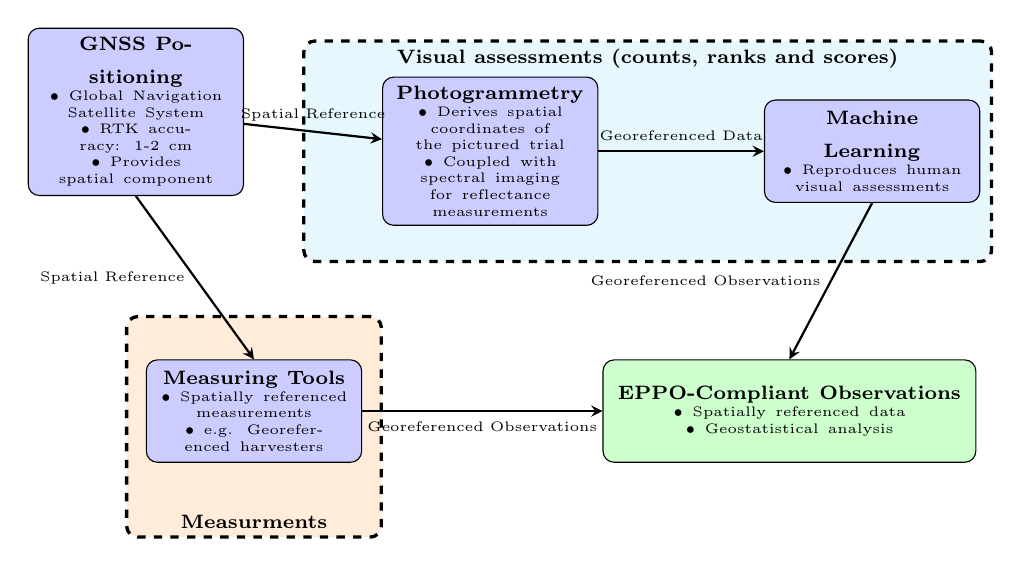
\begin{tikzpicture}[
            block/.style={rectangle, draw, fill=blue!20, text width=2.5cm, text centered, rounded corners, minimum height=1.3cm},
            arrow/.style={thick,->,>=stealth},
            groupbox/.style={rectangle, draw, rounded corners, very thick, dashed}
        ]
            
            % Background grouping rectangles
            % Light blue background for Visual assessments
            \node[groupbox, fill=cyan!10, text width=8.5cm, minimum height=2.8cm] (visual_group) at (5,0.5) {};
            \node[below] at (visual_group.north) {\scriptsize \textbf{Visual assessments (counts, ranks and scores)}};
            
            % Light orange background for Continuous values
            \node[groupbox, fill=orange!15, text width=3cm, minimum height=2.8cm] (continuous_group) at (0,-3) {};
            \node[above] at (continuous_group.south) {\scriptsize \textbf{Measurments}};
            
            % GNSS Block
            \node[block] (gnss) at (-1.5,1) {
                \textbf{\scriptsize GNSS Positioning}\\
                \tiny
                $\bullet$ Global Navigation Satellite System\\
                $\bullet$ RTK accuracy: 1-2 cm\\
                $\bullet$ Provides spatial component\\
            };
            
            % Spectral Photogrammetry Block
            \node[block] (photogrammetry) at (3,0.5) {
                \textbf{\scriptsize Photogrammetry}\\
                \tiny
                $\bullet$ Derives spatial coordinates of the pictured trial\\
                $\bullet$ Coupled with spectral imaging for reflectance measurements\\
            };
            
            % ML Inference Block
            \node[block] (ml) at (7.85,0.5) {
                \textbf{\scriptsize Machine Learning}\\
                \tiny
                $\bullet$ Reproduces human visual assessments\\
            };
            
            % Georeferenced Measuring Tools
            \node[block] (tools) at (0,-2.8) {
                \textbf{\scriptsize Measuring Tools}\\
                \tiny
                $\bullet$ Spatially referenced measurements\\
                $\bullet$ e.g. Georeferenced harvesters\\
            };
            
            % Output Block
            \node[block, fill=green!20, text width=4.5cm] (output) at (6.8,-2.8) {
                \textbf{\scriptsize EPPO-Compliant Observations}\\
                \tiny
                $\bullet$ Spatially referenced data\\
                $\bullet$ Geostatistical analysis\\
            };

            % Arrows with proper syntax
            \draw[arrow] (gnss) -- (photogrammetry) node[midway,above] {\tiny Spatial Reference};
            \draw[arrow] (photogrammetry) -- (ml) node[midway,above] {\tiny Georeferenced Data};
            \draw[arrow] (ml.south) -- (output.north) node[midway,left] {\tiny Georeferenced Observations};
            \draw[arrow] (gnss.south) -- (tools.north) node[midway,left] {\tiny Spatial Reference};
            \draw[arrow] (tools.east) -- (output.west) node[midway,below] {\tiny Georeferenced Observations};

        \end{tikzpicture}
    \end{center}

\end{frame}

\end{document}
